%! Author = Sujal Singh
%! Date = 11/3/23

% Preamble
\documentclass[12pt]{ipu-mechanics}
\title{Engineering Mechanics\\[10pt]Assignment--1}

% Packages
\usepackage{amsmath}
\usepackage{mathtools}
\usepackage[
    pdftitle={Engineering Mechanics Assignment 1},
    pdfsubject={Engineering Mechanics Assignment 1},
    pdfauthor={Sujal Singh},
    pdfdisplaydoctitle,
    hidelinks,
]{hyperref}
\usepackage{tikz}
\usepackage{wrapfig}
\usepackage{bm}
\usepackage{amssymb}

\usetikzlibrary{angles,arrows.meta}
\tikzset{>={Latex[scale=1.5,round]}}

% Document
\begin{document}
    \maketitle

    \headerline{Engineering Mechanics}{\textbf{\large Assignment--1}}{Sujal Singh}

    %------------------------------------------------------------------------------------------------------------------%
    %------------------------------------------------------------------------------------------------------------------%

    \question{Determine the resultant of two concurrent forces with the help of law of parallelogram forces.}
    \noindent Let $F_A$ and $F_B$ be two concurrent forces and $R$ be the resultant of the two forces:

    \begin{wrapfigure}[1]{r}{0.5\textwidth}
        \centering
        %! suppress = Quote
        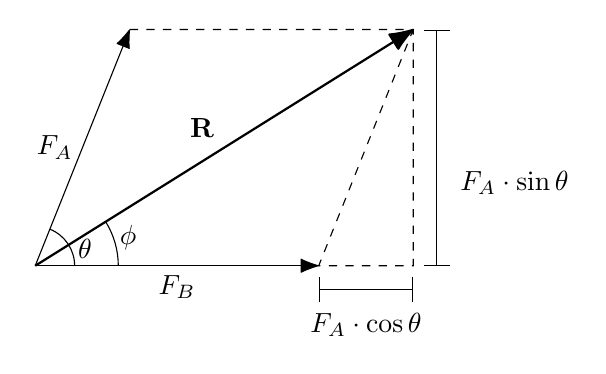
\begin{tikzpicture}[scale=0.6]
            % Forces
            \draw [<-] (2,5) coordinate (C) -- (0,0) node[midway,left] {$F_A$};
            \draw [->] (0,0) coordinate (B) -- (6,0) coordinate (A) node[midway, below] {$F_B$};
            \draw [->,thick] (0,0) -- (8,5) coordinate (D) node[midway,above left] {$\mathbf{R}$};

            \draw pic [draw] {angle=A--B--C} node[above=6pt,right=12pt] {$\theta$};
            \draw pic [draw,angle radius=30pt] {angle=A--B--D} node[above=10pt,right=27pt] {$\phi$};

            \draw [dashed] (2,5) -- (8,5) -- (6,0) -- (8,0) -- (8,5);
            \draw [{Bar[scale=2]}-{Bar[scale=2]}] (6,-0.5) -- (8,-0.5) node[midway,below=5pt] {$F_A\cdot\cos\theta$};
            \draw [{Bar[scale=2]}-{Bar[scale=2]}] (8.5,0) -- (8.5,5) node[midway,below right=5pt] {$F_A\cdot\sin\theta$};
        \end{tikzpicture}
    \end{wrapfigure}

    \begin{flalign*}
        R_x &= F_B + F_A\cdot\cos\theta &&\\
        R_y &= F_A\cdot\sin\theta
    \end{flalign*}
    By the Pythagorean Theorem,
    \begin{flalign*}
        R^2 &= {R_x}^2 + {R_y}^2 &&\\
        &= (F_B + F_A\cdot\cos\theta)^2 + {F_A}^2\cdot\sin^2\theta &&\\
        &= ({F_B}^2 + {F_A}^2\cdot\cos^2\theta + 2 F_B F_A\cdot\cos\theta) + {F_A}^2\cdot\sin^2\theta &&\\
        &= {F_B}^2 + {F_A}^2\cdot(\cos^2\theta + \sin^2\theta)+ 2 F_B F_A\cdot\cos\theta &&\\
        &= {F_A}^2 + {F_B}^2 + 2 F_A F_B\cdot\cos\theta
    \end{flalign*}
    $\therefore$~, the magnitude and direction of the resultant of the two forces is:\\

    % I don't know why the center environment isn't working
    % (it centers at half the width, as if the wrapfig hasn't ended)
    \parbox{\textwidth}{\centering
        $\boxed{\bm{R = \sqrt{{F_A}^2 + {F_B}^2 + 2 F_A F_B\cdot\cos\theta}}}$
        \\[10pt]
        $\tan\phi = \frac{R_y}{R_x}$
        \\[10pt]
        $\boxed{\bm{\phi = \tan^{-1}\left(\frac{R_y}{R_x}\right)}}$
    }
\end{document}